\begin{figure}[hbt!]
\centering
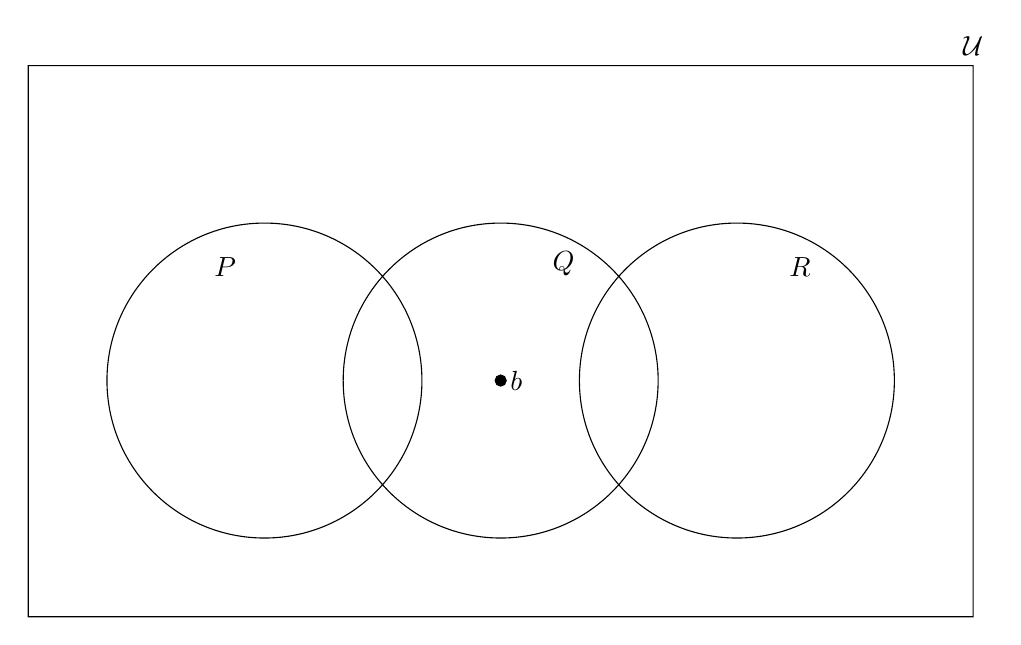
\begin{tikzpicture}[fill=gray]
      \draw ( 0,0 ) circle (2) (-0.5,1.2)  node [text=black,above] {$P$}
            ( 3,0 ) circle (2) (3.8,1.2)  node [text=black,above] {$Q$}
            ( 6,0 ) circle (2) (6.8,1.2)  node [text=black,above] {$R$}
            (-3,-3) rectangle (9,4) node [text=black,above] {$\mathcal U$};
      \filldraw[black] (3,0) circle (2pt) node[anchor=west] {$b$};
\end{tikzpicture}
\caption{Venn diagram for problem 1.1.1 \\
      - P: is the set of $x$ satisfies $p(x)$.\\
      - Q: is the set of $x$ satisfies $q(x)$.\\
      - R: is the set of $x$ satisfies $r(x)$.\\
      - $\exists b\in\mathcal U: p(b)\lor q(b), q(b)\lor r(b), \neg (p(b)\lor r(b))$ so given argument is invalid
}
\end{figure}